\documentclass[12pt]{article}
\usepackage{fontspec}
\setmainfont{Times New Roman}
\usepackage{graphicx}
\usepackage{dirtree}
\usepackage{hyperref}
\usepackage{graphicx}
\usepackage{float}
\usepackage{enumitem}
\usepackage{caption}
\usepackage[%
    left=1.5cm,    % Narrower left margin
    right=1.5cm,   % Narrower right margin
    top=2cm,       % Reduced top space
    bottom=3cm,    % More footer space
    headheight=15pt,
    footskip=30pt
]{geometry}
\usepackage{listings}
\usepackage{xcolor}
\usepackage{tikz}
\usetikzlibrary{positioning,shapes,shadows,arrows}

\definecolor{myblue}{RGB}{80,80,160}
\definecolor{mygreen}{RGB}{80,160,80}

\lstset{
    basicstyle=\small\ttfamily,
    keywordstyle=\color{myblue}\bfseries,
    commentstyle=\color{mygreen},
    breaklines=true,
    showstringspaces=false
}

\title{\textbf{Project Proposal: Travel Agency Management System}}
\author{Peter Jiang}
\date{\today}

\begin{document}

\maketitle

\section{Introduction}
This proposal outlines the development of a Travel Agency Management System. The system aims to streamline operations for travel agencies by providing a platform for managing travel bookings, itineraries, and customer information. The system will employ Object-Oriented Programming (OOP) principles, utilize file I/O for data persistence, and feature a user-friendly graphical interface built with Java Swing.

\section{Real-World Scenario and Business Logic}

\subsection{Scenario Overview}
The Travel Agency Management System serves the needs of a modern travel agency that offers various travel packages to different destinations. The agency handles customer bookings, maintains trip itineraries, manages payments, and collects customer reviews. This system will digitize these processes, enhancing efficiency and customer satisfaction.

\subsection{Business Logic}
The core business logic of the Travel Agency Management System includes:

\begin{itemize}
    \item \textbf{Customer Management}: Register new customers, update customer information, and track customer preferences and booking history.
    
    \item \textbf{Package Management}: Create, update, and delete travel packages with details such as destination, duration, accommodations, activities, and pricing.
    
    \item \textbf{Booking Process}: Allow customers to browse packages, make reservations, and process payments.
    
    \item \textbf{Itinerary Management}: Create and modify detailed day-by-day itineraries for each package or custom trip.
    
    \item \textbf{Review System}: Collect and display customer reviews and ratings for travel packages.
    
    \item \textbf{Reporting}: Generate reports on sales, popular destinations, and customer satisfaction metrics.
\end{itemize}

\section{Object-Oriented Design}

\subsection{Class Hierarchy}
The system will implement a robust class structure that leverages key OOP concepts including inheritance, polymorphism, interfaces, and abstract classes.

\subsection{UML Class Diagram}

\begin{figure}[H]
\centering
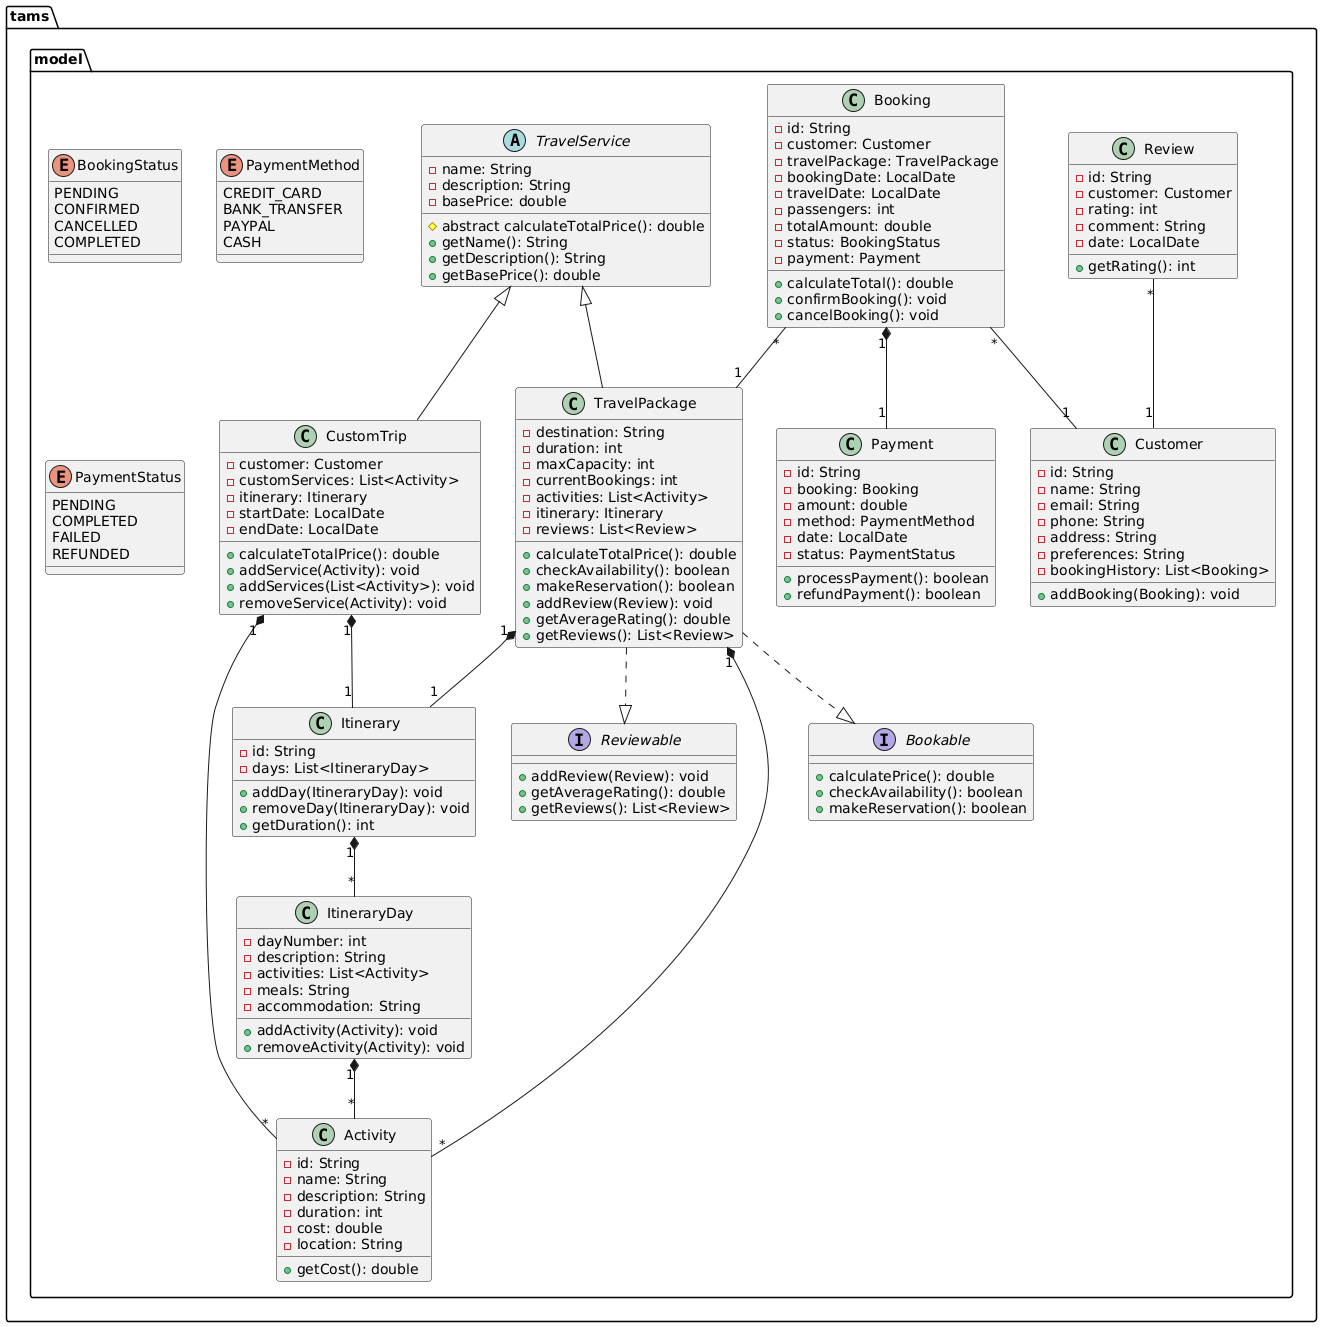
\includegraphics[width=\textwidth]{uml1.png}
\caption{UML Class Diagram for Travel Agency Management System}
\end{figure}
\newpage

\subsection{OOP Concepts Implementation}

\subsubsection{Interfaces}
The system implements two main interfaces:

\begin{itemize}
    \item \textbf{Bookable}: Defines methods that any bookable service must implement, including \texttt{calculatePrice()}, \texttt{checkAvailability()}, and \texttt{makeReservation()}.
    
    \item \textbf{Reviewable}: Defines methods for entities that can receive customer reviews, including \texttt{addReview()}, \texttt{getAverageRating()}, and \texttt{getReviews()}.
\end{itemize}

\subsubsection{Abstract Classes}
\begin{itemize}
    \item \textbf{TravelService}: An abstract class that provides common attributes and methods for all travel services. It includes abstract methods like \texttt{calculateTotalPrice()} that must be implemented by subclasses.
\end{itemize}

\subsubsection{Inheritance}
The inheritance hierarchy includes:
\begin{itemize}
    \item \texttt{TravelService} serves as the parent class for \texttt{TravelPackage} and \texttt{CustomTrip}.
    \item Each subclass inherits common attributes and methods while implementing specific behaviors.
\end{itemize}

\subsubsection{Polymorphism}
Polymorphism is demonstrated through:
\begin{itemize}
    \item Different implementations of \texttt{calculateTotalPrice()} in \texttt{TravelPackage} and \texttt{CustomTrip}.
    \item Use of the \texttt{Bookable} interface allowing different bookable services to be treated uniformly.
\end{itemize}

\subsubsection{Method Overloading}
\begin{itemize}
    \item Multiple constructors in classes like \texttt{Booking} and \texttt{Customer} with different parameter sets.
    \item \texttt{addService()} method in \texttt{CustomTrip} with versions for adding single services or collections.
\end{itemize}

\subsubsection{Method Overriding}
\begin{itemize}
    \item Override of \texttt{calculateTotalPrice()} in subclasses of \texttt{TravelService}.
    \item Override of \texttt{toString()} in various classes for customized string representation.
\end{itemize}

\subsubsection{Exception Handling}
Custom exceptions will include:
\begin{itemize}
    \item \texttt{BookingException}: For handling errors in the booking process, such as unavailable packages.
    \item \texttt{PaymentProcessException}: For managing payment processing errors.
\end{itemize}

\section{Graphical User Interface Design}

The GUI will be implemented using Java Swing, providing an intuitive interface for users to interact with the system.

\subsection{GUI Structure (Booking Panel)}

\begin{figure}[H]
\centering
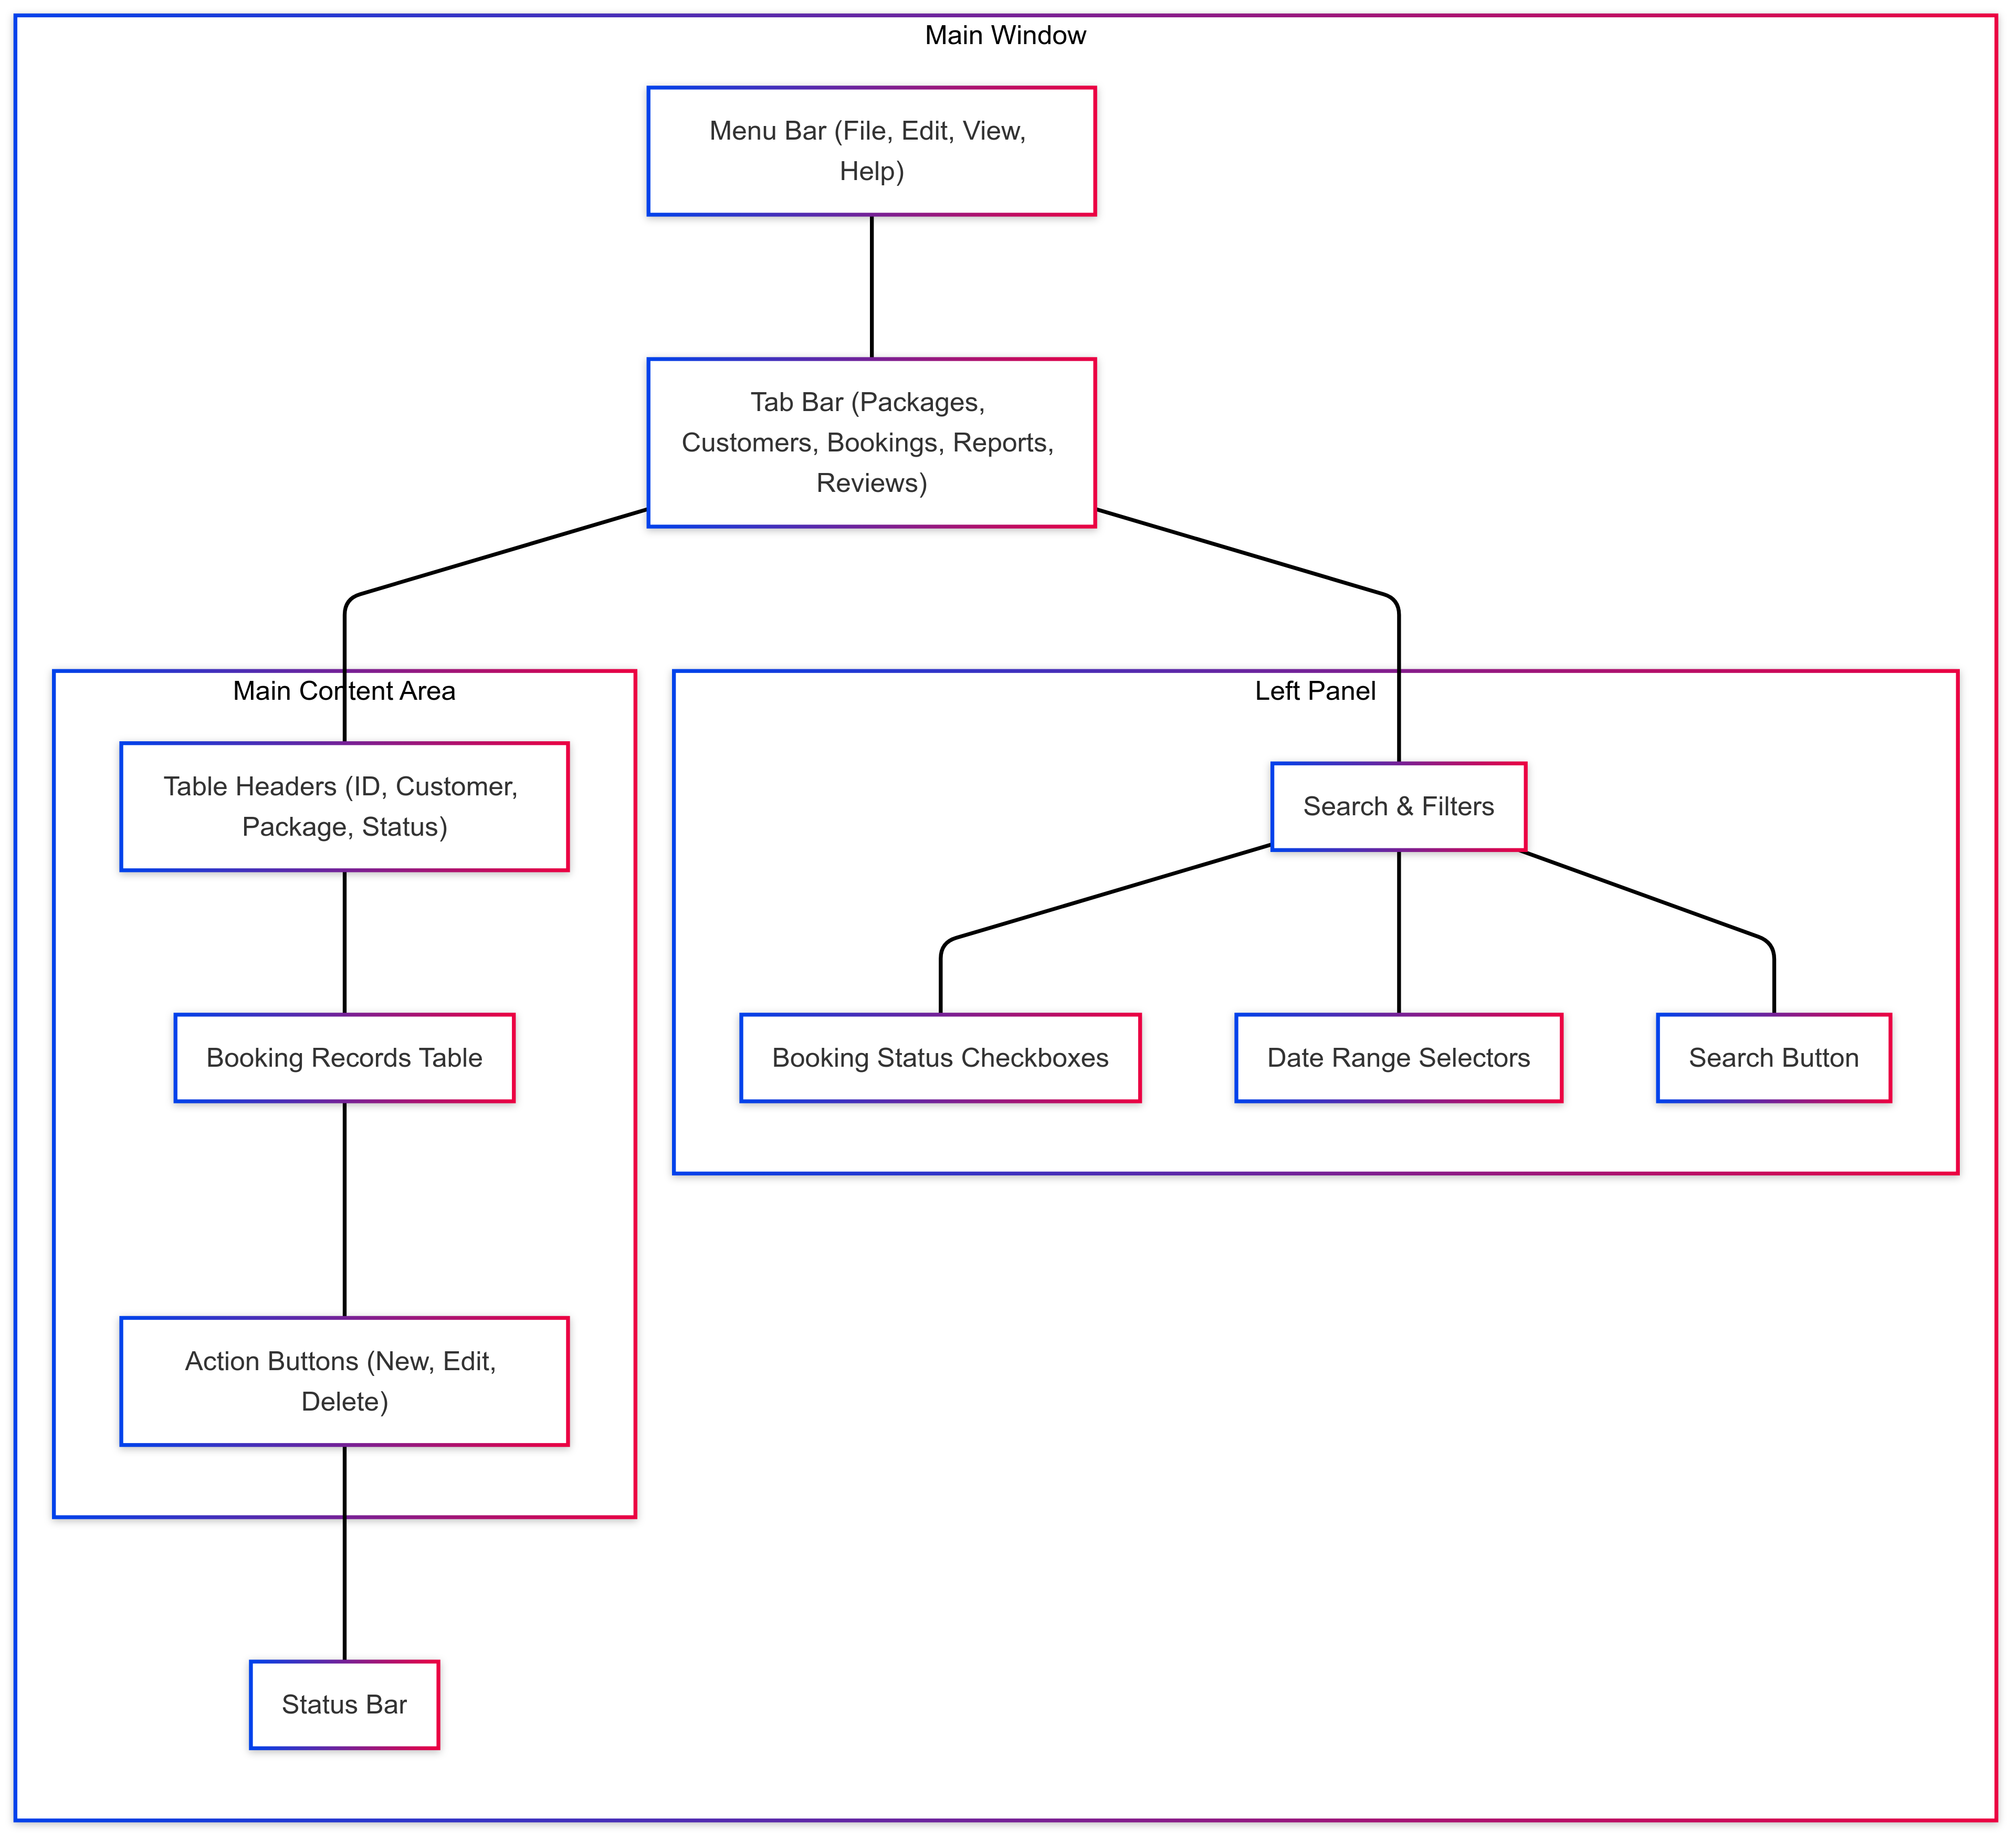
\includegraphics[width=\textwidth]{uml2.png}
\caption{GUI Structure (Booking Panel)}
\end{figure}
\newpage

\begin{figure}[H]
\centering
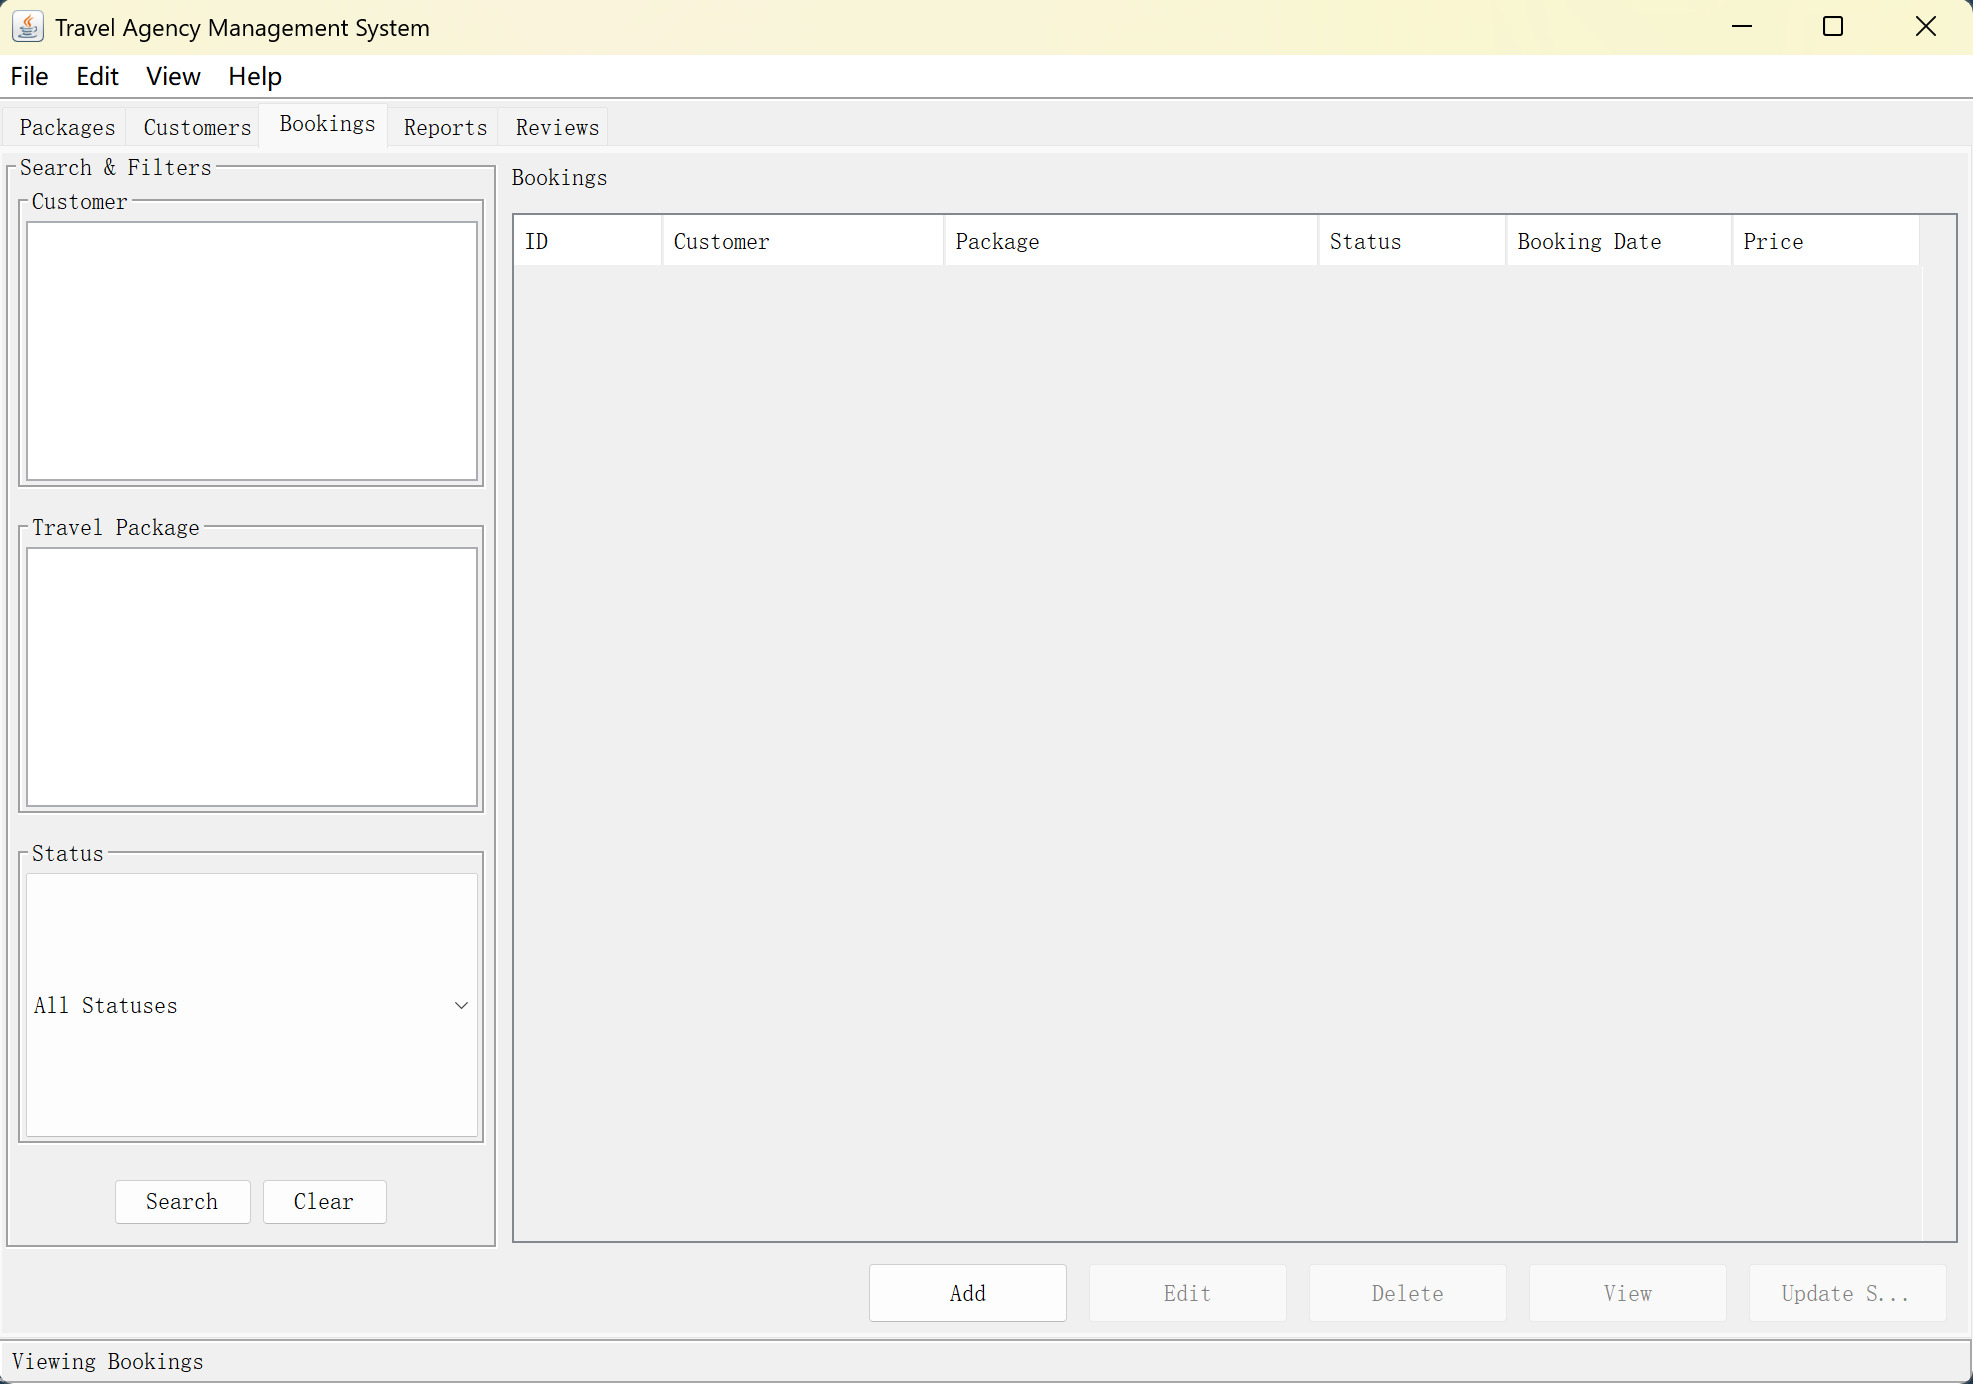
\includegraphics[width=\textwidth]{gui2.png}
\caption{Booking Panel}
\end{figure}
\newpage

\subsection{GUI Features}

The GUI will include the following features:

\begin{itemize}
    \item \textbf{Tab-based Navigation}: Easy navigation between different system functions (Packages, Customers, Bookings, Reports, Reviews).
    
    \item \textbf{Search and Filtering}: Ability to search and filter data across all modules.
    
    \item \textbf{CRUD Operations}: Interface elements for creating, reading, updating, and deleting records:
    \begin{itemize}
        \item \textbf{Create}: Forms to add new packages, customers, bookings, etc.
        \item \textbf{Read}: Tables and detailed views to display information.
        \item \textbf{Update}: Forms to modify existing records.
        \item \textbf{Delete}: Options to remove records with confirmation.
    \end{itemize}
    
    \item \textbf{Reports Section}: Visual representation of sales data, popular packages, and customer reviews.
    
    \item \textbf{Notification System}: Alerts for important events like booking confirmations or payment processing.
\end{itemize}

\section{Data Storage Design}

\subsection{File I/O Architecture}
The system will use file I/O to store and retrieve data persistently. The data storage will be organized as follows:

\begin{itemize}
    \item \textbf{JSON File Format}: Data will be stored in JSON format for readability and ease of handling.
    
    \item \textbf{File Structure}:
    \begin{itemize}
        \item \texttt{customers.json}: Customer information and preferences.
        \item \texttt{packages.json}: Travel package details and availability.
        \item \texttt{bookings.json}: Booking records and status.
        \item \texttt{reviews.json}: Customer reviews and ratings.
        \item \texttt{activities.json}: Available activities for packages.
    \end{itemize}
    
    \item \textbf{Data Loading}: When the application starts, it will load data from these files into memory.
    
    \item \textbf{Data Saving}: Changes will be saved back to the files when data is modified or when the application closes.
    
    \item \textbf{Backup Mechanism}: The system will create backups of data files periodically to prevent data loss.
\end{itemize}

\subsection{Data Processing}
The system will include:

\begin{itemize}
    \item \textbf{Data Validation}: Validating user inputs before saving to ensure data integrity.
    
    \item \textbf{Sorting and Searching}: Implementation of algorithms to efficiently sort and search through data collections.
    
    \item \textbf{Data Analysis}: Functions to analyze booking trends, popular destinations, and revenue statistics.
\end{itemize}

\section{Additional Features}

\subsection{Advanced Search Functionality}
The system will include advanced search options to:
\begin{itemize}
    \item Search packages by destination, date range, price range, or activities.
    \item Filter customer records by booking history or preferences.
    \item Search bookings by status, date, or package type.
\end{itemize}

\subsection{Data Analysis}
The system will offer data analysis features:
\begin{itemize}
    \item Monthly and yearly booking trends.
    \item Most popular destinations and packages.
    \item Customer spending patterns.
    \item Revenue forecasting based on booking data.
\end{itemize}

\section{Conclusion}
The proposed Travel Agency Management System will provide a comprehensive solution for travel agencies to manage their operations efficiently. By implementing the outlined features and following object-oriented design principles, the system will offer a robust, user-friendly platform that enhances the agency's ability to serve customers and track business performance.

The development will focus on creating a modular, maintainable system that fulfills all the requirements specified in the project guidelines, including OOP concepts, data storage, GUI implementation, and additional features for data analysis and advanced search functionality.

\end{document}